\section{Evaluations}
\label{sec:swapping_eval}

The goal of our evaluations is to compare the \eps generation rates, evaluate
the fidelity of generated \epss, and validate our analytical models.
We implement the various schemes over a discrete event simulator 
for QNs called NetSquid~\cite{netsquid2020}. 
The NetSquid simulator accurately models various QN components/aspects, and
%such as 
%physical hardware, fidelity, decoherence, photon transmission, gate/BSM operations,
%and propagation delays.
%%%%%%%%%%%%%%%%%%%%%%%%%%%%
in particular, we are able to 
define various QN components and simulate swapping-trees protocols
by implementing gate operations in entanglement swapping.  


\begin{figure}[ht]
    \centering
    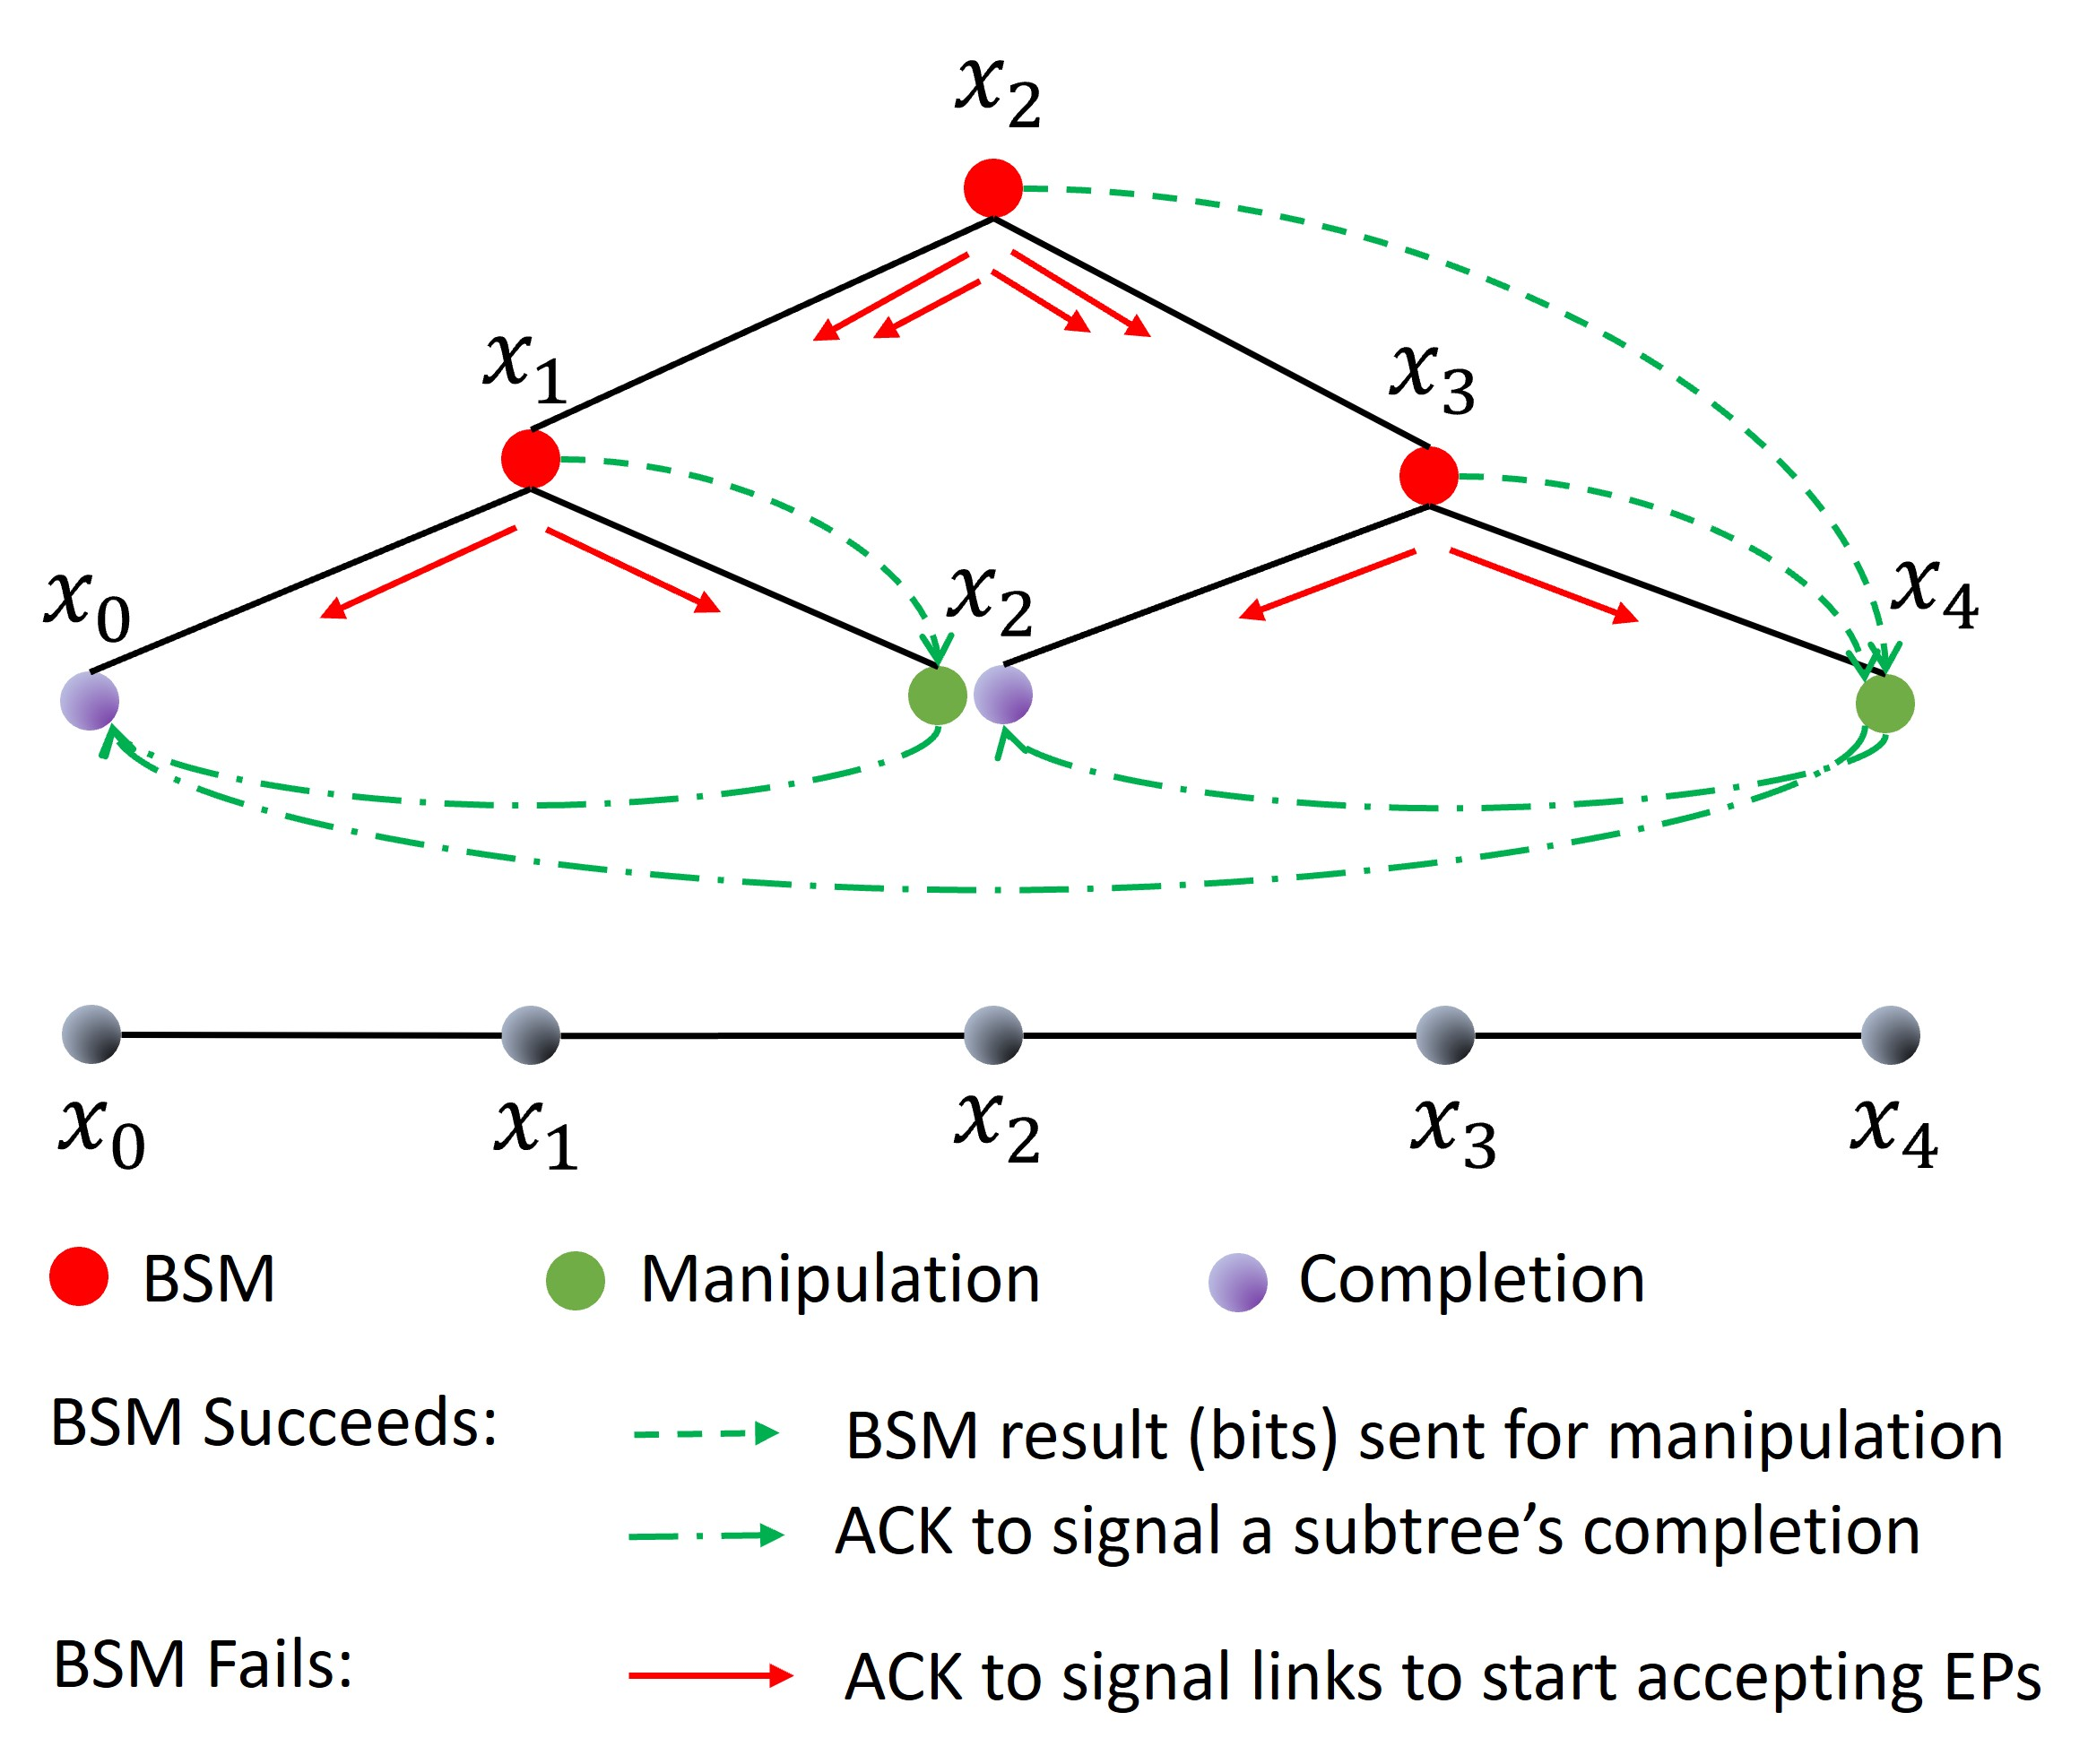
\includegraphics[width=0.8\textwidth]{chapters/swappingtrees/figures/protocol.jpg}
  \caption{Swapping Tree Protocol Illustration.
  The shown tree is a certain hierarchy of nodes to illustrate the BSM operation in the swapping-tree protocol.  
  A link-layer protocol continuously generates \epss over links $(x_0, x_2)$ and $(x_2, x_4)$.
  On receiving \eps on links on either side, $x_1$ ($x_3$) attempts a BSM operation on the stored
  qubit atoms. If the BSM succeeds, $x_1$ ($x_3$) sends two classical bits (solid green arrows) to  $x_2$ ($x_4$) 
  for desired manipulation/correction after which $x_2$ ($x_4$) sends an ACK (dashed green arrows) to the other end-node $x_0$ ($x_2$) to complete the EP generation. If 
  BSM  at  $x_1$ and $x_3$ are both successful, then $x_2$ attempts the BSM as above. 
  If a BSM at say $x_1$ fails, that $x_1$ failure signals (red arrows) to all the descendant nodes of the subtree
  rooted at $x_1$ so that they can start accept new \epss from the link layer protocol. 
  Note that here node $x_2$ plays multiple roles and hence appears at multiple places in the figure.}
  \label{fig:swapping_protocol}
\end{figure}

\para{Swapping Tree Protocol.}
Our algorithms compute swapping tree(s), and we need a way to implement them on a network. 
We build our protocol on top of the link-layer of~\cite{sigcomm19},
which is delegated with the task of continuously generating \epss on a link at a desired rate (as per the swapping tree specifications).
Note that a link $(a,b)$ may be in multiple swapping trees, and hence, may need to handle multiple link-layer requests 
at the same time; we implement such link-layer requests by creating independent atom-photon generators at $a$ and $b$, 
with one pair of synchronized generators for each link-layer request. 
As the links generate continuous \epss at desired rates, we need a protocol to
swap the \epss. Omitting the tedious bookkeeping details, the key aspect of the protocol
is that swap operation is done only when both the appropriate \eps pairs have arrived.
We implement all the gate operations (including, atomic and optical BSMs) within 
NetSquid to keep track of the fidelity of the qubits. 
On BSM success, the swapping node transmits classical bits to the end node which manipulates its qubit, and send the final ack to the other end node. 
On BSM failure, a classical ack is send to all descendant link leaves, so that they can now start accepting new link \epss; note that in our protocol, a link $l$ does not 
accept any more \epss, while its ancestor is waiting for its sibling's \eps. See Fig.~\ref{fig:swapping_protocol}.


\para{Simulation Setting.}
We use a similar setting as in the recent work~\cite{sigcomm20}.
%%%%%%%%%%
By default, we use a network spread over an area of $100 km \times 100 km$.
We use the Waxman model~\cite{waxman}, used to create Internet topologies,
to randomly distribute the nodes and create links; we use the maximum link
distance to be 10km. We vary the number of nodes from 25 to 
500, with 100
as the default value. We choose the two parameters in the Waxman model to
maintain the number of links to 3\% of the complete graph (to ensure an 
average degree of 3 to 15 nodes).
%%%%%%%%%%%%%%%%%%%%%%%%%%%%%%%%
For the \spp problem, we pick $(s,d)$ pairs within a certain range of
distance, with the default being 30-40 kms.
% for the \qnr problem, we extend this range to 10-70 kms. 



% \red{We pick parameters such that they are close to atom-photon entanglement; other type of quantum memories can also be used. The atomic memories can also be assumed in forms of ensemble especially as some second-long decoherence time has been achieved\cite{sagi10, vetsch10, deutsch10}.}
% \red{More specifically,} we use parameter values as the 
% ones used in~\cite{caleffi} \red{with an exception of decoherence time of 2 seconds}, and vary some
% of them. 

\softpara{Parameter Values.}
\blx{We use parameter values mostly similar to the ones used in~\cite{caleffi} corresponding to a single-atom based quantum memory platform, and vary some of them.}
In particular, we use atomic-BSM probability of success (\bp) 
to be 0.4 and latency (\bt) to be 10 $\mu$ secs; in some plots, we vary \bp from 
0.2 to 0.6. The optical-BSM probability of success (\php) is half of \bp. 
We use atom-photon generation times (\gt) and probability of success
(\gp) as 50 $\mu$sec and 0.33 respectively. Finally, we use photon 
transmission success probability 
as $e^{-d/(2L)}$~\cite{caleffi} where $L$ is the channel attenuation length
(chosen as 20km for an optical fiber) and $d$ is the distance between the nodes.
%%%%%%%%%%%%%%%%%%%%%%%%%%%%%%%%%%%%%
Each node's memory size is randomly chosen within a range of 15 to 20 units.
%%%%%%%%%%%%%%%%%%%%%%%%%%%
Fidelity is modeled in NetSquid using two parameter values, viz., depolarization
(for decoherence) and dephasing (for operations-driven) rates. 
%%%%%%%%%%%%%%%%%%%
We choose a decoherence time of two seconds based on achievable
values with single-atom memory platforms~\cite{loock20}; 
note that decoherence times of even several 
minutes~\cite{dec-13,dec-14} to hours~\cite{dec-15,dec-2021} has been 
demonstrated for other applicable memory platforms. 
Accordingly, we choose a depolarization rate of 0.01 such that the 
fidelity after a second is 90\%.
Similarly, we choose a dephasing rate of 1000 which corresponds to a link \eps 
fidelity of 99.5\%~\cite{delft-lp}.

%\red{Finally, we conservatively discard qubits/EPs that age more than a second.}

% \begin{figure}
%     \centering
%     \includegraphics[width=0.5\textwidth]{resources/figures/fidelity.jpg}
%     \vspace{-0.0in}
%     \caption{ (a) \eps  Rates, and (b) Fidelity, over linear \blue{paths.} \red{Distance --> Length}}
%     \vspace{-0.05in}
%     \label{fig:fidelity}
% \end{figure}

% \begin{figure}
%     \centering
%     \includegraphics[width=0.5\textwidth]{resources/figures/line_extra.jpg}
%     \vspace{-0.0in}
%     \caption{\red{Make 11(b) to 10(c) with times upto 60 seconds. Make 11(a) to 10 (d), and change the text accordingly.}}
%     \vspace{-0.05in}
%     \label{fig:line_extra}
% \end{figure}


\para{Algorithms and Performance Metrics.}
To compare our techniques with prior approaches, we implement most recently proposed
approaches, viz., (i) \blx{the \os-based \tqbl{linear programming (LP)} approach 
from~\cite{delft-lp} (called
\delftlp here), (ii) \qcast approach from~\cite{sigcomm20} which is \os-based but
uses multiple links and requires memories.} 
The \wt-based algorithm
by Caleffi~\cite{caleffi} uses an
exponential-time approach, and is thus compared only for small networks.
The~\cite{guha} and~\cite{greedy2019distributed} approaches are not compared
as they were found to be inferior to \qcast.
Alrorithms \dpo and \dpa in~\cite{swapping-tqe-22} are also being compared.
We compare our \dpalt with all the above mentioned algorithms largely in terms of \eps generation rates and the execution times.

For all algorithm except for \qcast, we use only one link between adjacent nodes,
since only \qcast takes advantage of multiple links in a creative way. 
%%%%%%%%%%
In particular, for \qcast, we use $W = 1, 5$, or 10 sub-links (\cite{sigcomm20} calls them
channels) on each link, with the node and link "capacity" divided equally among the 
them.
\eat{(e.g., for $W=5$ sub-links, each node's atom-photon generation capacity is divided among
$2W = 10$ sub-links to handle sub-links on either side).}
%%%%%%%%%%%%
We note that in \qcast each node requires $2W$ memories (2 for each sub-link)
with sufficient coherence time to allow for the entire swapping operation over the
path to be completed.
%%%%%%%%%%%%%%%%%%%%%%
The \delftlp approach explicitly assumes the generation of link \epss is deterministic,
i.e., the value $\gp^2\ep^2\php$ is 1, and does not model node generation rates. 
We address these differences by 
extending their LP formulation: (i) We add a constraint on node generation
rates, and (ii) add a $\gp^2\ep(i,j)^2\php$ factor to each link $(i,j)$ in any path
extracted from their LP solution.
% Among our schemes, we use \dpo, \dpa and \dpalt (see \S\ref{sec:swapping_efficient}) for the \spp problem.
% We compare the schemes largely in terms of \eps generation rates; we also
% compare the execution times and \epss fidelity.

\begin{figure}[t]
    \centering
    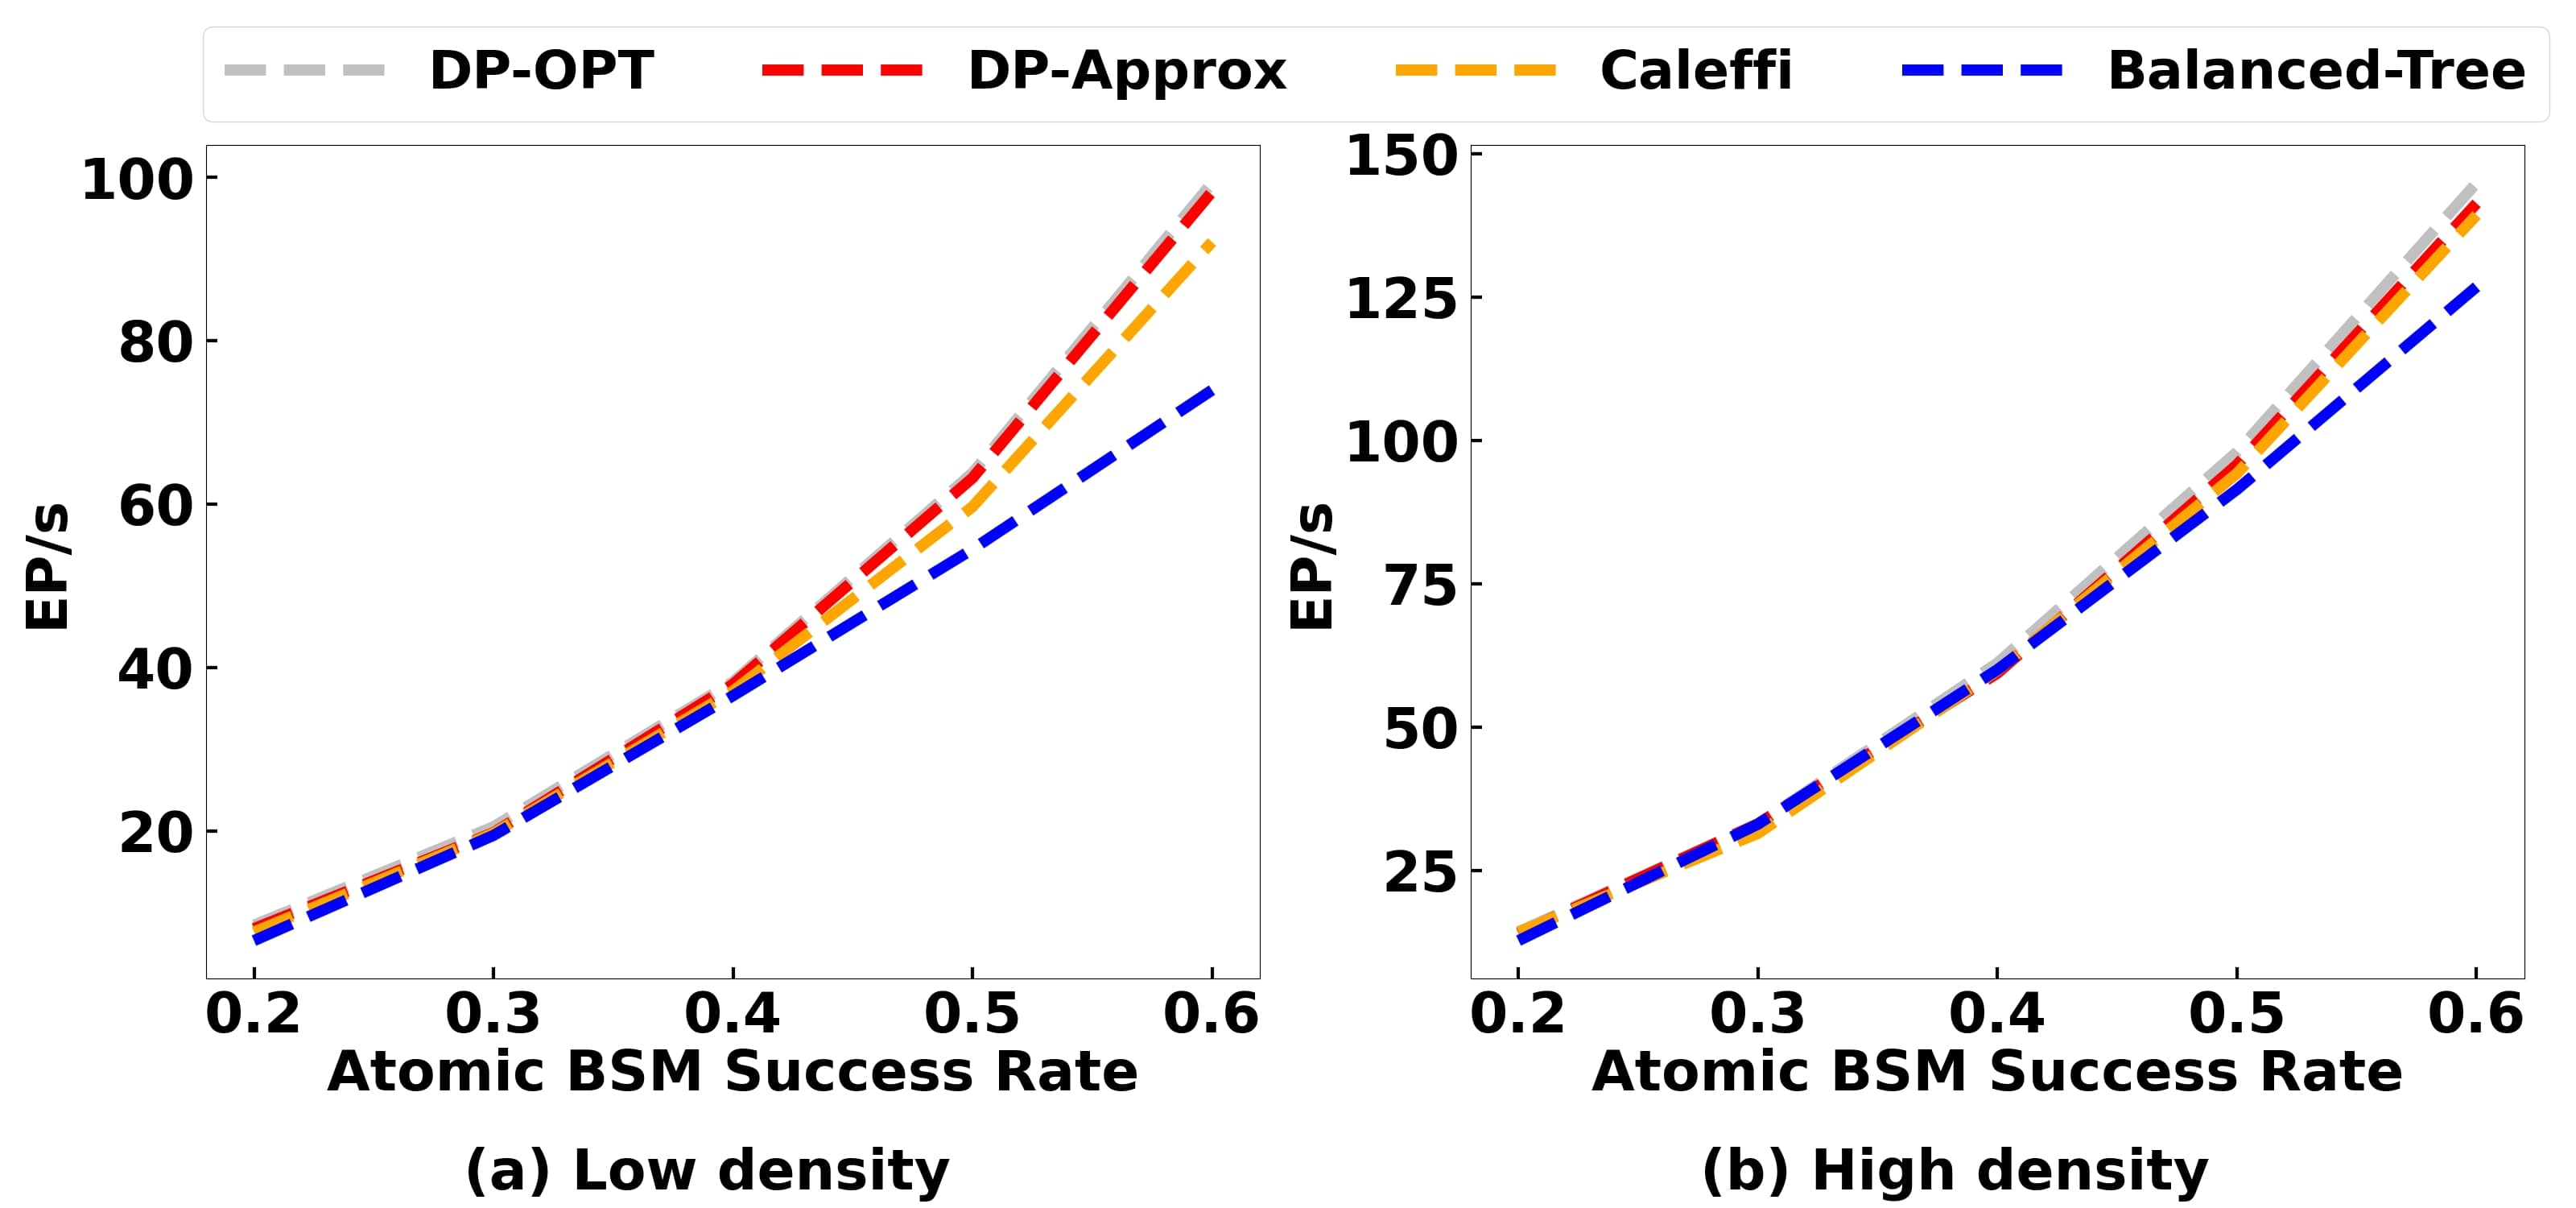
\includegraphics[width=0.9\textwidth]{chapters/swappingtrees/figures/caleffi.jpg}
    % \vspace{-0.0in}
    \caption{Compare the performance with Caleffi in a (a) low density network and a (b) high density network.}
    % \vspace*{-0.05in}
    \label{fig:swapping_caleffi}
\end{figure}

\para{Comparison with~\cite{caleffi} for \spp Problem.}
Note that~\cite{caleffi} gives only an \spp algorithm referred to as
\clf; it takes
exponential-time making it infeasible to run for
network sizes much larger than 15-20. In particular, for network sizes
17-20, it takes several hours, and our preliminary analysis suggests that
it will take of the order of $10^{40}$ \textit{years} on our 100-node
network. See Table~\ref{tab:swapping_runtime}.
%%%%%%%
Thus, we use a small network of 15 nodes over a 25km $\times$ 25km area;
we consider average node degrees of 3 or 6. See Fig.\ref{fig:swapping_caleffi}.
%%%%%%%%
We see that \dpo outperforms \clf by 10\% on a average for the sparser
graph and minimally for the denser graph. 
% However, for some instances, \dpo outperformed \clf by as much as 300\% (see Appendix~\ref{app:swapping_clf-perf}). 
We see that \dpa performs similar to \dpo,
while \dpalt is outperformed slightly by \clf; however, for this small
network, since the \dpo and \dpa algorithms only take 10-100s of
msecs (Table~\ref{tab:swapping_runtime}), \dpalt need not be used in practice.  
%%%%%%%%%%%%%%%%%%%%%%

\eat{
notably better than~
We see that each node has a degree of 3 on average, the performance of \dpa is almost 10\% better than Caleffi on average. We pick $(s,d)$, randomly. In cases, where even the best $(s,d)$ pairs' path are at least four hops and the difference between balanced vs. non-balanced comes to the picture, the performance difference between our \dpo (or even \dpa) than ~\cite{caleffi} is more substantial. See Fig.[??]. This difference can be as high as 3 times as Fig.~\ref{fig:non-balance} shows.
In Fig.~\ref{fig:caleffi}(b), a high density case, where each node has 6 neighbors, \dpa is still better than Caleffi, but the margin is smaller. 
The performance of \dpalt is inferior to Caleffi. 
}


\begin{figure*}[t]
    % \vspace{-0.0in}
    \centering
    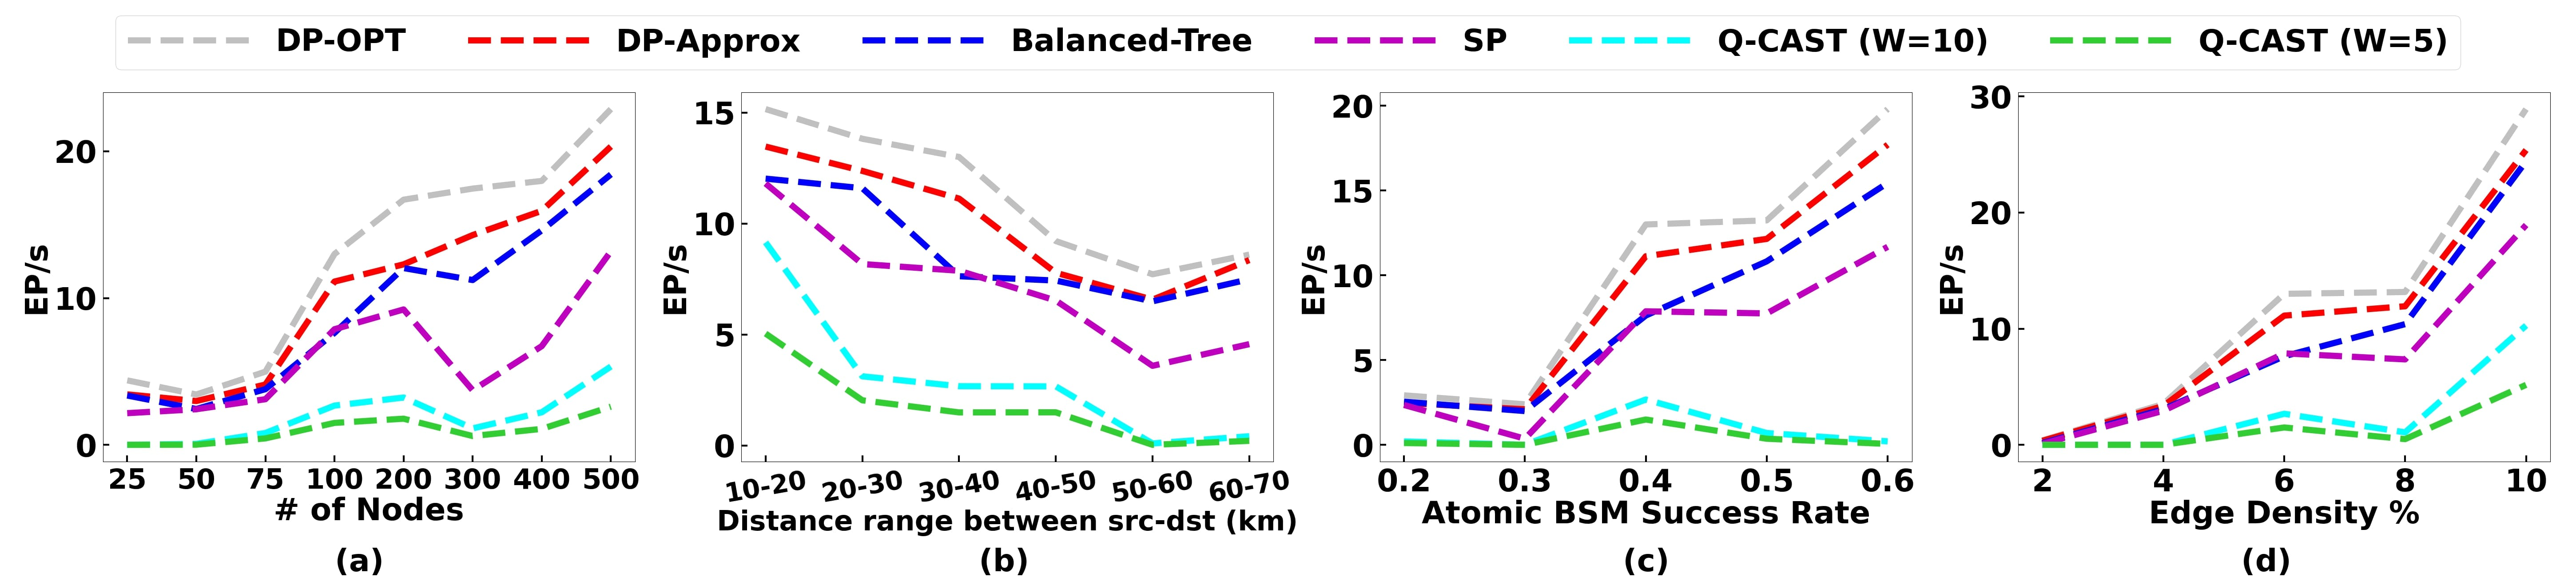
\includegraphics[width=\textwidth]{chapters/swappingtrees/figures/QNR-SP.jpg}
    % \vspace{0.0in}
    \caption{\spp Problem: \eps Generation Rates for varying parameters.}
    % \vspace{-0.05in}
    \label{fig:swapping_spp}
\end{figure*}

\begin{figure}
    \centering
    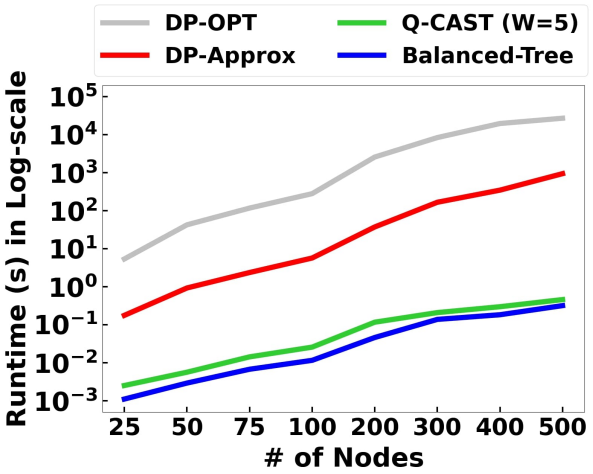
\includegraphics[width=0.5\textwidth]{chapters/swappingtrees/figures/runtime-sp.png}
    % \vspace{-0.1in}
    \caption{The execution time comparison of various algorithms for \spp algorithms.}
    \label{fig:swapping_runtime}
\end{figure}




% \begin{figure*}[t]
%     % \vspace{-0.0in}
%     \centering
%     \includegraphics[width=\textwidth]{figures/swappingtrees/QNR.jpg}
%     % \vspace{-0.0in}
    
%     \caption{\qnr Problem: \eps Generation Rates for varying parameters.}
%     \label{fig:swapping_qnr}
%     % \vspace{-0.05in}
% \end{figure*}


\sloppypar
\para{\spp Problem (Single Tree) Results.}
We start with comparing various schemes for the \spp problem, in terms of \eps generation
rate. We compare \dpa, \dpo, \dpalt, \naive, and \qcast; 
% note that the LP schemes can't be used to select a \textit{single} tree, as they turn into ILPs. 
%%%%%%%%
See Fig.~\ref{fig:swapping_spp}, where we plot the \eps generation rate for various schemes for
varying number of nodes, $(s, d)$ distance, \bp, and network
link density. We observe that \dpa and \dpo perform very closely, with the \dpalt heuristic
performing close to them; all these three schemes outperform the \qcast schemes (for $W=5, 10$ sub-links) by an 
order of magnitude. We don't plot \qcast for $W=1$ sub-links, 
as it performs much worse (less than $10^{-3}$ \eps/sec).
%%%%%%%%
We note that \qcast's \eps rates here are much lower than the ones published in~\cite{sigcomm20}, because~\cite{sigcomm20} uses link \eps success 
probability of 0.1 or more, while in our
more realistic model, the link \eps success probability is 
$\gp^2\ep^2\php = 0.012$ for the default \bp value.
%%%%%%%%%%%%%%%%%%%%%%%%%%%%%%%%%
We reiterate that our schemes require only 2 memory 
units per node, while the \qcast schemes requires $2W$ units. 
\eat{In addition, \qcast and \delftlp require 
tight synchronization of all links across a path, while
our schemes are asynchronous.}
%%%%%%%%%%%%%%%%%%%%%%%%%%%
The main reason for poor performance of \qcast (in spite of higher memory and link synchronization) 
is that, in the \os model, the \eps generation
over a path is a very low probability event---essentially $p^l$ where $p$ is the link-\eps success probability and $l$ is the path length, for the case of $W=1$
(the analysis for higher $W$'s is involved~\cite{sigcomm20}).
\blx{Finally, our proposed techniques also outperform the \naive algorithm, especially when the number of possible paths (trees) between $(s,d)$ pair increases.}
%%%%%%%%%%%%%%%%%%%%%%%%%%%%%%%%%%%
In addition, 
%Other than the above key observations, 
we see that performance increases with increase in \bp, number of nodes, or network link density, as expected due to availability of better trees/paths; it also increases with decrease in $(s,d)$ distance as fewer hops are needed.
%The performance increases with increase in \bp, and decreases  with increase in $(s,d)$ distance as more hops are needed. 

% \para{\qnr Problem Results.}
% We now present performance comparison of various schemes for the \qnr problem. Here, we compare
% the following schemes: \iterdpa, \iterdpalt, \iternaive, \delftlp, and \qcast \bleu{with the optimal \LP as the benchmark for comparison (\LP wasn't feasible to run
% for more than 100 nodes).}
% %%%%%%%%%%%%%%%%%%%%%
% See Fig.~\ref{fig:swapping_qnr}. Our observations are similar to that for the \spp problem results. 
% We see that in all plots, \LP being optimal performs the best, but is closely matched by
% \iterdpa and the efficient heuristic \iterdpalt.
% \blx{We observe that  the performance gap between our proposed techniques and \iternaive is higher than in the \spp case, as \naive picks paths based on just number of 
% links.}
% Our schemes outperform both \delftlp and \qcast
% by an order of magnitude, for the same reason as mentioned above. 

% \begin{figure*}
%     \centering
%     \includegraphics[width=\textwidth]{figures/swappingtrees/line_extra2.jpg}
%     % \vspace{-0.0in}
%     \caption{\eps generation over linear paths. 
%     (a) \eps  Rates, and (b) Fidelity, over linear paths with varying link lengths. 
%     (c) Maximum reachable distance with links of 30-35m lengths.
%     (d) \eps generation rates over linear paths with 10-50 km links to demonstrate impact of varying link lengths.}
%     % \vspace{-0.05in}
%     \label{fig:swapping_fidelity}
% \end{figure*}



% \para{Fidelity and Long-Distance Entanglements.}
% We now investigate the fidelity of the \epss generated. 
% First, we note that the \qcast and \delftlp schemes will incur near-zero decoherence 
% as they involve only transient storage. 
% Decoherence for other schemes is also negligible as the \eps generation 
% latencies (10s of msecs) is much less than the coherence time. 
% %%%%%%%%%%%%%
% The operations-driven fidelity loss is expected to be similar for all schemes, as they
% all roughly use the same order of links. 
% %%%%%%%%%%%%%
% Overall, we observed fidelities of 94-97\% across all schemes (not shown), 
% with our schemes also
% performing better sometimes due to smaller number of leaves.

% \softpara{Long Path Graphs.}
% To test the limits of the schemes in terms of decoherence and fidelity, 
% we consider a long path network and estimate fidelity of \epss generated by
% schemes for increasing distances and link-lengths (link success probability 
% decreases with increasing link length).
% %%%%%%%
% %%%%%%%%%%%%%%%%%%%%%%%%%%%%%%%%%%%
% Fig.~\ref{fig:swapping_fidelity}(a)-(b) shows \eps generation rates and fidelity for path lengths
% of 500km and 1000km for varying link lengths, for the single-tree schemes \dpa and \dpalt. \qcast and \delftlp are not shown as their \eps rate is near-zero ($\leq 10^{-20}$) 
% at these distances. 
% We observe that our schemes yield \epss 
% with qubit fidelities of 65-82\% and 40-64\% for 500km and 1000km paths respectively, 
% with \eps rates of 0.05 to 0.65/sec. These are viable results---since 
% \blue{qubit copies with fidelities higher than 50\% can be purified 
% to smaller copies with 
% arbitrarily higher fidelities~\cite{bennett-95,bennett-96}.}

% \blx{
% Now, in Fig.~\ref{fig:swapping_fidelity}(c), we demonstrate the effect of decoherence time of quantum memories used in nodes.
% Here, we use 30-35 km links. We see that even with decoherence time of as low as 100 ms, \dpa is able to create \epss for up to 200 kms while \dpalt can only create \eps for paths up to~120 kms; they perform similarly for larger
% decoherence times.
% As all the links are almost of the same length, the optimal swapping will be largely-balanced trees wherein the \eps generation rate depends only on the 
% tree height. Due to this reason, the maximum achievable path-length graph is 
% close to a step function.
% We add that our schemes produce 0.008 \epss/s for distance of more than 4000 kms.}

% \blx{
% Finally, in Fig.~\ref{fig:swapping_fidelity}(d), we demonstrate the higher performance of non-balanced trees when the links
% on a path may have much different lengths. In particular, we pick link lengths randomly in the range of 10 to 50 kms. With this setting, we see that \dpa performs much better than \dpalt, and in some cases, up to 100\% better. 
% Note that, \dpalt and \clf have similar performance over linear graphs, as there is no path selection scheme needed.}

\eat{
We observe that .. 
%%%%%%%%%%%%%%%%%%%%%%%%%%%%%
Fig.~\ref{fig:fidelity}(a) shows fidelity and \eps generation rates for varying
$(s,d)$ path lengths with link length in the range of 30-35 km, 
and Fig.~\ref{fig:fidelity}(d) shows fidelity and \eps generation rates for path length
of 500km with varying link length.}

% \begin{figure*}
% %  \vspace{-0.04in}
%     \centering
%     \includegraphics[width=\textwidth]{figures/swappingtrees/analytical_throttle.jpg}
%     % \vspace{-0.025in}
%     \caption{Comparing with Analytical Results. (a) Analytical vs.\ Simulation Results. (b) Throttled vs.\ Non-Throttled Trees (\spp). (c) Throttled vs.\ Non-Throttled Trees (\qnr). (d) Fairness Measure.}
%     % \vspace{-0.025in}
%     \label{fig:swapping_analytical}
% \end{figure*}

% \para{Validating the Analysis; Fairness.}
% %We now evaluate the accuracy of our analytical results. 
% Fig.~\ref{fig:swapping_analytical}(a) compares the \eps generation rates as measured by the analytical formulae and the actual simulations for the \spp algorithms \dpa and \dpalt. We observe that they
% match closely, validating our assumption of 3/2 factor in 
% Eqn.~\ref{eqn:swapping_tree-rate}
% % Eqn.~\ref{eqn:tree-rate} 
% and of exponential distributions at higher levels of the tree, and of the path metric $M()$ for \dpalt.
% %%%%%%%%%%%%%%%
% Fig.~\ref{fig:swapping_analytical}(b)-(c) plots the \eps generation rates for throttled and non-throttled trees. We see that the throttled tree 
% underperforms the non-throttled tree by only a small margin for the single-tree case; however,
% for the multi-tree \iterdpalt algorithm,
% the throttled trees perform better as they are able to use the resources efficiently. 
% %%%%%
% Fig.~\ref{fig:swapping_analytical}(d) plots the average number of $(s,d)$ pairs that get at least one
% tree/path for varying number of requests; we see that our schemes exhibit 
% 90-99\% fairness.


% \cbl
\para{Execution Times.}
We ran our simulations on an Intel i7-8700 CPU machine, and observed that  the \os algorithms as well our \dpalt and \iterdpalt
heuristics run in fraction of a second even for a 500-node network; thus,
they can be used in real-time. Note that since our problems depend on real-time network state (residual capacities), 
the algorithms must run very fast.
The other algorithms (viz., \dpo, \dpa, and \iterdpa) can take minutes to hours on large networks, and hence, may be impractical on large network 
without significant optimization and/or parallelization. See Fig~\ref{fig:swapping_runtime}.


\begin{table*}[ht]
    \centering
    \caption{Execution times of \spp algorithm over small networks} %title of the table
    % \centering % centering table
    \begin{tabular}{c rrrrrr} % creating 8 columns
    \hline\hline %inserting double-line
    Algorithm&\multicolumn{6}{c}{Number of nodes} \\ [0.5ex]
    & 10 & 13 & 15 & 16 & 18 & 20 \\
    \hline % inserts single-line
    \dpalt & 239$\mu$s & 360$\mu$s & 373$\mu$s& 492$\mu$s& 530$\mu$s& 552$\mu$s\\
    \dpa & 4ms & 10ms & 14.7ms& 17.6ms& 28ms& 34ms\\
    \dpo & 148ms & 363ms & 572ms & 706ms& 1s& 1.7s\\ 
    Caleffi~\cite{caleffi} & 92ms & 4.6s & 14s& 26mins & 3.2hrs& 12.8hrs\\[1ex] % [1ex] adds vertical space
    \hline % inserts single-line
    \end{tabular}
    \label{tab:swapping_runtime}
\end{table*}
        
    
Here, we give execution times of different algorithms especially \clf's for small networks of 10-20 nodes.
 See Table~\ref{tab:swapping_runtime}. We see that \dpalt and \dpa take fractions of a second, while \dpo takes upto 2 seconds.
However, as expected \clf's execution time increases exponentially with increase in number of nodes -- 
with 20-node network takes 10+ hours. Below, we further estimate \clf's execution time for larger graphs.
% \para{Rough Estimate of \clf's Execution Time for Large Graphs.}
% Consider a $n$-node network with an average node-degree of $d$. Consider a node pair $(s,d)$. 
% We try to estimate the number of paths from $s$ to $d$ -- the goal here is merely to show that the number is astronomical 
% for $n$ = 100, and thus, our analysis is very approximate (more accurate analysis seems beyond the scope of this work). 
% %%%%%%%%%%%%%%%
% Let $P(l)$ be the number of simple paths from $s$ to a node $x$ in the graph of length at most $l$. For large graphs and 
% large $l$, we can assume $P(l)$ to be roughly same for all $x$. We estimate that $P(l+1) = P(l) + P(l)*6*(1 - l/n)$. 
% The first term is to count paths of length at most $l-1$; in the second term, the factor 6 comes from the fact the destination $x$ has 6 neighbors and the factor $(1-l/n)$ is the probability that a path counted in $P(l)$ doesn't contain $x$ (to constrain the paths to be simple, i.e,. without cycles). 
% %%%%%%%%%%%%%%%
% Using $P()$, the execution time of \clf can be roughly estimated to be at least $P(n-1)*500/(5*10^9)$ seconds where the 
% factor 500 is a conservative estimate of the number of instructions used in computing the latency for a path 
% and $5*10^{9}$ is the number of instructions a 5GHz machine can execute in a second.
% %%%%%%%%%%%
% The above yields executions times of a few seconds for $n=15$, 
% about an hours for $n=20$,  
% about 350 hours for $n=25$, 
% and $10^{16}$ hours for $n=50$,
% and $10^{44}$ hours for $n=100$. 
% The above estimates for $n=15$ to 20 are within an order of 
% magnitude of our 
% actual execution times, and thus, validate our estimation approach.
    

\eat{
\dpalt has the lowest runtime, with merely 0.0011 seconds in a 25 node network and 0.31 seconds in a 500 node network. 
\dpa takes from seconds to minutes and \dpo takes up to hours.
Fig.~\ref{fig:swapping_runtime}(b) shows the runtime of four algorithms for the \qnr problem.
\iterdpalt is the fastest and \iterdpa is the slowest.
In both \spp and \qnr problems, \qcast is only a little slower than our path heuristic.
\delftlp is slower than \qcast, and note that we used a package called OR-Tools by Google, which is written in C++ and is more efficient than our Python written code.
In summary, our path heuristic are the fastest and all the \os algorithms come next. 
And our DP based algorithms are the slowest. 
}


